\section{Metodología}

En esta sección presentaremos la metodología utilizada para la generación de HMMs, la interpolación entre los mismos y otras técnicas utilizadas.

A modo de resumen, estos serán los pasos a realizar:

\begin{enumerate}

\item A partir de tres corpus de datos, dos de ellos en castellano y uno en ingles, se realizará un etiquetado fonético de los corpus para su posterior utilización en el entrenamiento de los HMMs.

\item Realizar el entrenamiento de los sistemas (Uno por cada corpus disponible). Para esto contaremos con el framework de modelado de HMMs HTS. 

\item Una vez generados los HMMs utilizaremos herramientas provistas por HTS para interpolar entre ellos y así obtener distintos grados de fonética y prosodia inglesa a la hora de sintetizar audios.

\end{enumerate}

Dado que el castellano y el ingles no utilizan los mismos símbolos fonéticos, si queremos sintetizar audios en castellano con el HMM generado con el corpus en ingles, un desafío que deberemos resolver es el de cubrir todos los símbolos fonéticos del castellano por alguno del ingles.

\subsection{Preparación De los datos}

Como ya adelantamos, en este trabajo contamos con tres corpus de datos disponibles:

\begin{itemize}
\item secyt-mujer: 741 oraciones, $48$ minutos de habla.
\item loc1\_pal: 1593 oraciones, $2$ horas y $26$ minutos de habla.
\item CMU-ARCTIC-SLT: 1132 oraciones, 56 minutos de habla.
\end{itemize}

Para los tres corpus se contaba ademas con sus transcripciones grafemicas. 

Para poder realizar el entrenamiento con HTS, fue necesario generar los utternaces respectivos para cada corpus. Los mismos consisten basicamente en una transcripción fonetica de los audios dividida en segmentos temporales y metadata contextual como la cantidad de silabas en la palabra siendo transcripta, fonemas que preceden y proceden al actual, etc. Estos utternaces serán utilizados para modelar cada fonema con una mezcla de variables aleatorias gaussianas. 

Dadas la cantidad de horas de audio disponibles, y al costo que conlleva realizar transcripciones manuales de un corpus, tanto para loc1\_pal como para CMU-ARCTIC-SLT se decidió utilizar alineamiento forzado automático para obtener los utternaces mencionados. Para esto se utilizaron Festival y Festvox que a partir de los audios y sus transcripciones grafemicas, permite realizar EHMM alignment sobre el corpus de datos. Para secyt-mujer contábamos previamente con las transcripciones fonéticas realizadas a mano, por lo que primero probamos realizar un etiquetado con EHMM alignment, y luego un metodo mixto donde utilizambamos parte de la información del EHMM (principalmente para determinar que fonema correspondía en cada segmento) y las transcripciones a mano para ajustarlos de manera mas presisa.

Comparando resultados, el modelo generado con secyt-mujer y EHMM resulto ser el modelos que peor resultados arrojó, sintetizando oraciones con muchos clicks y voces mas metalicas. El metodo mixto si bien arrojó resultados mejores, todavía presentaba algunos clicks y una voz no del todo natural. Los mejores resultados fueron obtenidos por loc1\_pal con EHMM. Nuestra teoría es que esto se debe a la disparidad en la cantidad de audios y horas de habla. Concideramos que esto juega un papel predominante en la calidad de los TTS generados, aún cuando se utiliza un metodo de etiquetado puramente automatico y propenso a errores.

Para este trabajo todos los audios usarán sampling rate de 48kHz, precisión de 16 bits, mono.

% Cosas para hablar:
% 5 fonemas.
%TODO: phonetically balanced?
% desarrollar generacion de uternaces: secty alineaminento mixto: tiempos a mano, features automaticos.

\subsection{Repertorio Fonetico y Mapeo De Fonemas}

%hablar un poco mas de utternaces.

Para las transcripciones foneticas, tanto de los audios en ingles como en castellano, utilizamos los repertorios foneticos brindados por festvox (ver apendice 1).

El primer desafío que se presenta es que estos repertorios foneticos no tienen un mapeo directo con el Alfaveto Fonetico Internacional: por ejemplo con este repertorio fonetico, en el castellano existen tres fonemas distintos para la /i/. Consideramos que esta decición por parte de festvox proviene de la necesidad de poder diferenciar la /i/ acentuada de la no acentuada y de aquella presente en los diptongos. 

Por otra parte, surge aquí un problema: como sintetizar oraciones en castellano utilizando un repertorio fonetico distinto, donde incluso la cantidad de fonemas es diferente. Como solución a esto desarrollamos de manera perceptual e iterativa, un mapeo del ingles al castellano en el que cubriremos cada fonema del castellano por al menos uno del ingles. El mapeo que concideramos devolvió los mejores resultados puede observarse en el apendice.

Los fonemas marcados como notUsed los consideramos lo suficientemente diferentes como para no mapearse a nigun fonema del castellano.

Ademas para completar el repertorio, se tomaron la mitad de los fonemas /r/ y se remplazaron con /rr/ y de manera similar se tomaron la mitad de los fonemas etiquetados como /hh/ y se remplazaron con /g/.

Utilizamos este mapeo para generar un tts en ingles capaz de sintetizar oraciones en castellano. Por supuesto los resultados obtenidos sintetizando audios de esta manera generan audios incomprensibles y de muy baja calidad.

En el proximo paso procederemos a realizar mezclas entre el tts en castellano y el tts presentado aquí para generar un nuevo tts donde se pueda hacer un ajuste gradual de cada uno de estos modelos. 

% mapeo utilizado mostrar.
% el etiquetado de cmu\_arctic es en ingles y mapeando al castellano.

\subsection{Entrenamiento Con HTS}

HTS es un TTS basado en HMMs que modela simultáneamente la duración, el espectro (mel-cepstrum) y la frecuencia principal ($f0$) de manera simultanea utilizando un framework de HMM:

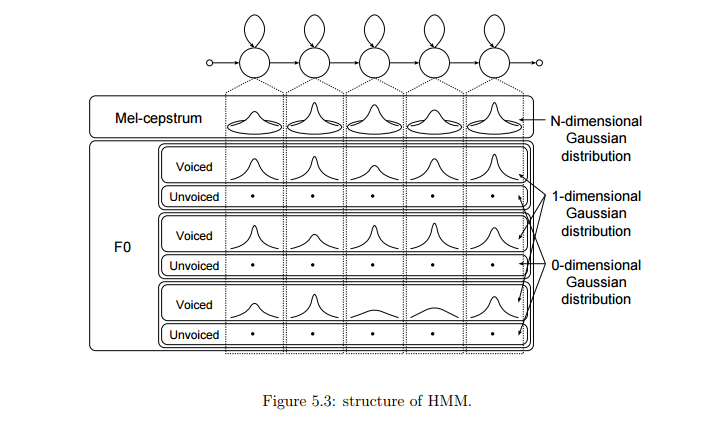
\includegraphics[scale=0.5]{imagenes/hmm.png}

Por otra parte HTS toma la decisión de modelar la información prosódica dentro de este mismo framework. Para esto, las distribuciones para el espectro, la frecuencia principal y las duraciones son clusterizadas independientemente utilizando la información contextual conseguida en los utternaces. A continuación se presenta una vista esquemática de la estructura de este HMM:

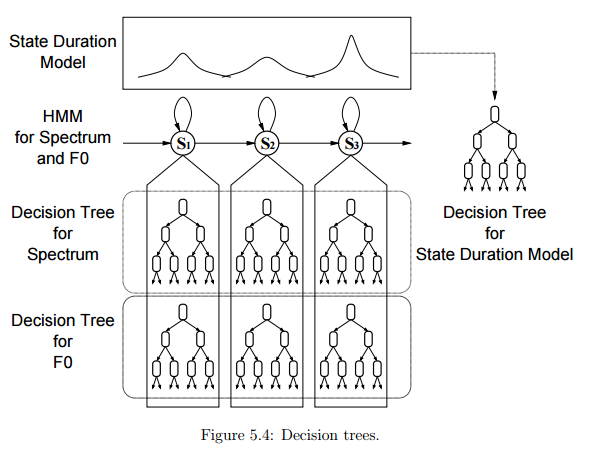
\includegraphics[scale=0.5]{imagenes/hmmContext.png}

En particular para este trabajo la clusterización de datos se realizó generando arboles de decición, para cada fonema se tomaron los dos fonemas precedentes y los dos fonemas procendetes y se extrageron las siguientes features:

\begin{itemize}
\item Modo de articulación del fonema.
\item Punto de articulación del fonema.
\item La perspectiva articulatoria (anterior, central o posterior).
\item Si el fonema es una vocal o una consonante.
\item En caso de ser una vocal, a que categoría pertenecía: por ejemplo para el fonema $/i/: {i, i0,i1}$.
\item En caso de ser una vocal, su Redondeamiento vocálico.
\item En caso de ser una consonante, si es lennis o fortis.
\end{itemize}

Esta información fué introducida con posterioridad al modelo, y pudimos apreciar una drastica mejora en los audios generados. Las primeras pruebas sonaban sumamente metalicas y carentes de prosodia pero una vez agregados los factores contextuales pudimos comprobar que ahora las voces sonaban mucho mas humanas.


(Aclarar: Imágenes extraídas de la disertación doctoral, Profesor Tadashi Kitamura)
% Cosas para hablar:
% contextual factors: cuales son, para que sirven.
% arboles de decición.
% questions
% expandir sobre hmms
\subsection{Síntesis utilizando hts\_engine}

Para la síntesis se utilizó hts\_engine, una herramienta de linea de comandos que no solo permite sintetizar oraciones utilizando los modelos acústicos generados sino además interpolar entre los distintos HMMs disponibles. Utilizaremos esta herramienta para interpolar entre los HMMs de ingles y castellano para lograr nuevos modelos que mezclen los features acústicos con distintos grados de ingles y de castellano.

Un desafío que se presenta para este trabajo es el mapeo de los fonemas del ingles al castellano. Para empezar, la transcripción fonética realizada por festival de las oraciones en ingles puede utilizar $50$ símbolos distintos, mientras que la transcripción fonética del castellano utiliza $31$. Habiendo además muchos símbolos sin equivalencia. (por ejemplo, con el fonema $\/rr$).

Para resolver esto desarrollamos una solución adhoc que consistió en desarrollar una función sobreyectiva que permita tener cubiertos los $31$fonemas del castellano por alguno del ingles.

% Cosas para hablar:
% Expandir en que consiste la interpolación.